\documentclass{standalone}
\usepackage{tikz}
\usetikzlibrary{patterns, positioning}

\begin{document}
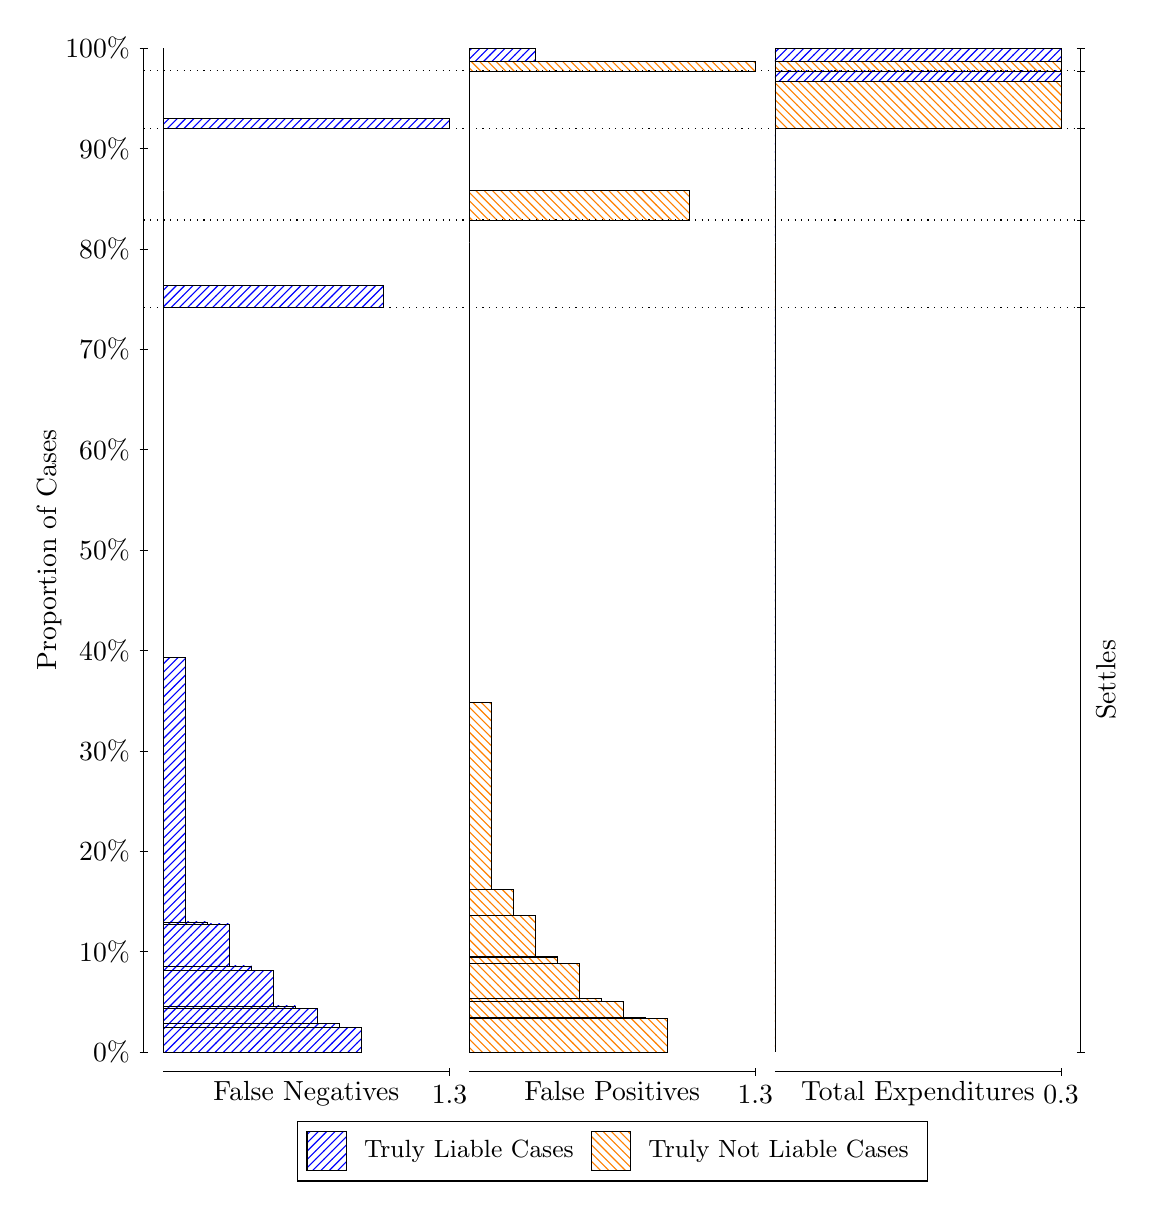
\begin{tikzpicture}
\draw[black, very thin] (1.5,1.75) -- (1.5,14.5);
\node[rotate=90, anchor=center] at (0.3, 8.125) {Proportion of Cases};
\draw[black, very thin] (1.45,1.75) -- (1.55,1.75);
\node[anchor=east] at (1.45, 1.75) {0\%};
\draw[black, very thin] (1.45,3.025) -- (1.55,3.025);
\node[anchor=east] at (1.45, 3.025) {10\%};
\draw[black, very thin] (1.45,4.3) -- (1.55,4.3);
\node[anchor=east] at (1.45, 4.3) {20\%};
\draw[black, very thin] (1.45,5.575) -- (1.55,5.575);
\node[anchor=east] at (1.45, 5.575) {30\%};
\draw[black, very thin] (1.45,6.85) -- (1.55,6.85);
\node[anchor=east] at (1.45, 6.85) {40\%};
\draw[black, very thin] (1.45,8.125) -- (1.55,8.125);
\node[anchor=east] at (1.45, 8.125) {50\%};
\draw[black, very thin] (1.45,9.4) -- (1.55,9.4);
\node[anchor=east] at (1.45, 9.4) {60\%};
\draw[black, very thin] (1.45,10.675) -- (1.55,10.675);
\node[anchor=east] at (1.45, 10.675) {70\%};
\draw[black, very thin] (1.45,11.95) -- (1.55,11.95);
\node[anchor=east] at (1.45, 11.95) {80\%};
\draw[black, very thin] (1.45,13.225) -- (1.55,13.225);
\node[anchor=east] at (1.45, 13.225) {90\%};
\draw[black, very thin] (1.45,14.5) -- (1.55,14.5);
\node[anchor=east] at (1.45, 14.5) {100\%};

\draw[black, very thin] (13.4,1.75) -- (13.4,14.5);
\draw[black, very thin] (13.35,1.75) -- (13.45,1.75);
\node[anchor=west] at (13.35, 1.75) {};
\draw[black, very thin] (13.35,11.202) -- (13.45,11.202);
\node[anchor=west] at (13.35, 11.202) {};
\draw[black, very thin] (13.35,12.316) -- (13.45,12.316);
\node[anchor=west] at (13.35, 12.316) {};
\draw[black, very thin] (13.35,13.479) -- (13.45,13.479);
\node[anchor=west] at (13.35, 13.479) {};
\draw[black, very thin] (13.35,14.21) -- (13.45,14.21);
\node[anchor=west] at (13.35, 14.21) {};
\draw[black, very thin] (13.35,14.5) -- (13.45,14.5);
\node[anchor=west] at (13.35, 14.5) {};

\draw[black, very thin, pattern color=blue, pattern=north east lines] (1.75,1.75) rectangle (4.2654,2.0594);
\draw[black, very thin, pattern color=blue, pattern=north east lines] (1.75,2.0594) rectangle (3.9859,2.1177);
\draw[black, very thin, pattern color=blue, pattern=north east lines] (1.75,2.1177) rectangle (3.7064,2.3018);
\draw[black, very thin, pattern color=blue, pattern=north east lines] (1.75,2.3018) rectangle (3.4269,2.3039);
\draw[black, very thin, pattern color=blue, pattern=north east lines] (1.75,2.3039) rectangle (3.4269,2.3362);
\draw[black, very thin, pattern color=blue, pattern=north east lines] (1.75,2.3362) rectangle (3.1474,2.789);
\draw[black, very thin, pattern color=blue, pattern=north east lines] (1.75,2.789) rectangle (2.8679,2.8429);
\draw[black, very thin, pattern color=blue, pattern=north east lines] (1.75,2.8429) rectangle (2.5885,3.3763);
\draw[black, very thin, pattern color=blue, pattern=north east lines] (1.75,3.3763) rectangle (2.309,3.4008);
\draw[black, very thin, pattern color=blue, pattern=north east lines] (1.75,3.4008) rectangle (2.0295,6.7584);
\draw[black, very thin, pattern color=orange, pattern=north west lines] (1.75,6.7584) rectangle (1.75,11.202);
\draw[black, very thin, pattern color=blue, pattern=north east lines] (1.75,11.202) rectangle (4.5449,11.484);
\draw[black, very thin, pattern color=orange, pattern=north west lines] (1.75,11.484) rectangle (1.75,12.316);
\draw[black, very thin, pattern color=orange, pattern=north west lines] (1.75,12.316) rectangle (1.75,12.688);
\draw[black, very thin, pattern color=blue, pattern=north east lines] (1.75,12.688) rectangle (1.75,13.479);
\draw[black, very thin, pattern color=blue, pattern=north east lines] (1.75,13.479) rectangle (5.3833,13.607);
\draw[black, very thin, pattern color=orange, pattern=north west lines] (1.75,13.607) rectangle (1.75,14.21);
\draw[black, very thin, pattern color=orange, pattern=north west lines] (1.75,14.21) rectangle (1.75,14.335);
\draw[black, very thin, pattern color=blue, pattern=north east lines] (1.75,14.335) rectangle (1.75,14.5);
\draw[black, very thin, pattern color=orange, pattern=north west lines] (5.6333,1.75) rectangle (8.1487,2.1785);
\draw[black, very thin, pattern color=orange, pattern=north west lines] (5.6333,2.1785) rectangle (7.8692,2.1924);
\draw[black, very thin, pattern color=orange, pattern=north west lines] (5.6333,2.1924) rectangle (7.5897,2.3878);
\draw[black, very thin, pattern color=orange, pattern=north west lines] (5.6333,2.3878) rectangle (7.3103,2.4304);
\draw[black, very thin, pattern color=orange, pattern=north west lines] (5.6333,2.4304) rectangle (7.0308,2.8732);
\draw[black, very thin, pattern color=orange, pattern=north west lines] (5.6333,2.8732) rectangle (6.7513,2.9499);
\draw[black, very thin, pattern color=orange, pattern=north west lines] (5.6333,2.9499) rectangle (6.7513,2.9624);
\draw[black, very thin, pattern color=orange, pattern=north west lines] (5.6333,2.9624) rectangle (6.4718,3.4801);
\draw[black, very thin, pattern color=orange, pattern=north west lines] (5.6333,3.4801) rectangle (6.1923,3.8175);
\draw[black, very thin, pattern color=orange, pattern=north west lines] (5.6333,3.8175) rectangle (5.9128,6.1931);
\draw[black, very thin, pattern color=blue, pattern=north east lines] (5.6333,6.1931) rectangle (5.6333,11.202);
\draw[black, very thin, pattern color=orange, pattern=north west lines] (5.6333,11.202) rectangle (5.6333,12.033);
\draw[black, very thin, pattern color=blue, pattern=north east lines] (5.6333,12.033) rectangle (5.6333,12.316);
\draw[black, very thin, pattern color=orange, pattern=north west lines] (5.6333,12.316) rectangle (8.4282,12.688);
\draw[black, very thin, pattern color=blue, pattern=north east lines] (5.6333,12.688) rectangle (5.6333,13.479);
\draw[black, very thin, pattern color=orange, pattern=north west lines] (5.6333,13.479) rectangle (5.6333,14.081);
\draw[black, very thin, pattern color=blue, pattern=north east lines] (5.6333,14.081) rectangle (5.6333,14.21);
\draw[black, very thin, pattern color=orange, pattern=north west lines] (5.6333,14.21) rectangle (9.2667,14.335);
\draw[black, very thin, pattern color=blue, pattern=north east lines] (5.6333,14.335) rectangle (6.4718,14.5);
\draw[black, very thin, pattern color=orange, pattern=north west lines] (9.5167,1.75) rectangle (9.5167,6.1931);
\draw[black, very thin, pattern color=blue, pattern=north east lines] (9.5167,6.1931) rectangle (9.5167,11.202);
\draw[black, very thin, pattern color=orange, pattern=north west lines] (9.5167,11.202) rectangle (9.5167,12.033);
\draw[black, very thin, pattern color=blue, pattern=north east lines] (9.5167,12.033) rectangle (9.5167,12.316);
\draw[black, very thin, pattern color=orange, pattern=north west lines] (9.5167,12.316) rectangle (9.5167,12.688);
\draw[black, very thin, pattern color=blue, pattern=north east lines] (9.5167,12.688) rectangle (9.5167,13.479);
\draw[black, very thin, pattern color=orange, pattern=north west lines] (9.5167,13.479) rectangle (13.15,14.081);
\draw[black, very thin, pattern color=blue, pattern=north east lines] (9.5167,14.081) rectangle (13.15,14.21);
\draw[black, very thin, pattern color=orange, pattern=north west lines] (9.5167,14.21) rectangle (13.15,14.335);
\draw[black, very thin, pattern color=blue, pattern=north east lines] (9.5167,14.335) rectangle (13.15,14.5);
\draw[black, dotted] (1.5,11.202) -- (13.4,11.202);
\draw[black, dotted] (1.5,12.316) -- (13.4,12.316);
\draw[black, dotted] (1.5,13.479) -- (13.4,13.479);
\draw[black, dotted] (1.5,14.21) -- (13.4,14.21);
\draw[black, very thin] (1.75,1.5) -- (5.3833,1.5);
\node[anchor=north] at (3.5667, 1.5) {False Negatives};
\draw[black, very thin] (5.3833,1.45) -- (5.3833,1.55);
\node[anchor=north] at (5.3833, 1.45) {1.3};

\draw[black, very thin] (5.6333,1.5) -- (9.2667,1.5);
\node[anchor=north] at (7.45, 1.5) {False Positives};
\draw[black, very thin] (9.2667,1.45) -- (9.2667,1.55);
\node[anchor=north] at (9.2667, 1.45) {1.3};

\draw[black, very thin] (9.5167,1.5) -- (13.15,1.5);
\node[anchor=north] at (11.333, 1.5) {Total Expenditures};
\draw[black, very thin] (13.15,1.45) -- (13.15,1.55);
\node[anchor=north] at (13.15, 1.45) {0.3};

\node[black, centered, rotate=90] at (13.72, 6.4758) {Settles};





\draw (7.449999999999999,1.5) node[draw=none] (baseCoordinate) {};
\begin{scope}[align=center]
        \matrix[scale=0.5, draw=black, below=0.5cm of baseCoordinate, nodes={draw}, column sep=0.1cm]{
            \node[rectangle, draw, minimum width=0.5cm, minimum height=0.5cm, pattern=north east lines, pattern color=blue] {}; &
            \node[draw=none, font=\small] (B) {Truly Liable Cases}; &
            \node[rectangle, draw, minimum width=0.5cm, minimum height=0.5cm, pattern=north west lines, pattern color=orange] {}; &
            \node[draw=none, font=\small] (B) {Truly Not Liable Cases}; \\
            };
\end{scope}

\end{tikzpicture}
\end{document}